\documentclass[xcolor=table,presentation]{beamer}    % ,handout
% colortbl only defines \rowcolor for a single row. xcolor extends this to multiple rows.

\usetheme[sectionoutline]{Aachen} %
\usepackage[ngerman]{babel}
\usepackage[T1]{fontenc}
\usepackage[utf8]{inputenc}


%%%%%%%%%%%%%%%%%%%%%%%%%%%%%%%%%%%%%%%%%%%%%%%%%%%%%%%%%%%%%%%%%%%%%%
% tables
\usepackage{multirow,array,tabularx,rotating}
\usepackage{booktabs}

% math
\usepackage{amsmath,amsthm, amssymb, latexsym, xspace}
\usepackage{bbold}
%\usefonttheme[onlymath]{serif}
%\boldmath

% misc
\usepackage{subfigure}
\usepackage{wasysym}
\usepackage{nameref}

\usepackage{tikz}
\usetikzlibrary{trees,calc}
\usepackage[absolute,overlay]{textpos}

\tikzset{
grow=down,
level 1/.style={sibling distance=7cm, level distance=3cm},
level 2/.style={sibling distance=7cm, level distance=3cm},
level 3/.style={sibling distance=7cm, level distance=3cm},
level 4/.style={sibling distance=7cm, level distance=3cm},
edge/.style={thick},
edge from parent path={
(\tikzparentnode) |-
($(\tikzparentnode)!0.5!(\tikzchildnode)$) -|
(\tikzchildnode)},
}

\tikzstyle{end} = [circle, minimum width=5pt, fill, inner sep=0pt]

\renewcommand*\ttdefault{txtt}


% declare the path(s) where your graphic files are
\graphicspath{./bilder/}
% and their extensions so you won't have to specify these with
% every instance of \includegraphics
\DeclareGraphicsExtensions{.pdf,.jpeg,.png}

% helpers
\newcommand{\argmin}{\operatornamewithlimits{argmin}}
\newcommand{\argmax}{\operatornamewithlimits{argmax}}

%%%%%%%%%%%%%%%%%%%%%%%%%%%%%%%%%%%%%%%%%%%%%%%%%%%%%%%%%%%%%%%%%%%%%%
%%%%%%%%%%%%%%%%%%%%%%%%%%%%%%%%%%%%%%%%%%%%%%%%%%%%%%%%%%%%%%%%%%%%%%

\renewcommand*{\email}{\url{thomas.gatzweiler@rwth-aachen.de}}
% all email address(es) of the authors (used for \TitlePage)

\title[Adaptive Huffman-Kodierung und Anwendungen]{Adaptive Huffman-Kodierung und Anwendugen}

\setbeamertemplate{navigation symbols}{} %disable navigation bar

%% author and in []: shortauthor
\author[Gatzweiler]{Thomas Gatzweiler}
% - Use the \inst{?} command only if the authors have different
%   affiliation.
\institute[RWTH Aachen University] % (optional, but mostly needed)
{
%  \inst{1}%
  \strut Human Language Technology and Pattern Recognition\\
  \strut Computer Science Department, RWTH Aachen University %\\
  %\strut {\tt lehnen@cs.rwth-aachen.de}
}
% - Use the \inst command only if there are several affiliations.
% - Keep it simple, no one is interested in your street address.

\date[12. November 2014]{Proseminar Datenkompression, 12. November 2014, Aachen}

%%%%%%%%%%%%%%%%%%%%%%%%%%%%%%%%%%%%%%%%%%%%%%%%%%%%%%%%%%%%%%%%%%%%%%
% will be set into the PDF document summary
\hypersetup{
  pdftitle={\inserttitle}, 
  pdfauthor={\insertauthor}, 
  bookmarksdepth=subsubsection,  
  % enable automatic page transitions: for endless loop edit in
  % acrobat reader -> preferences -> full screen -> after every X
  % seconds and after last page
  %pdfpageduration = 2, 
  % pdfpagetransition = {Glitter /Di 315 /D 5}  
  % pdfpagetransition = {Box /M /O /D 1},
}

%%%%%%%%%%%%%%%%%%%%%%%%%%%%%%%%%%%%%%%%%%%%%%%%%%%%%%%%%%%%%%%%%%%%%%
\usepackage{pdfpcnotes}

%%%%%%%%%%%%%%%%%%%%%%%%%%%%%%%%%%%%%%%%%%%%%%%%%%%%%%%%%%%%%%%%%%%%%%
%%%%%%%%%%%%%%%%%%%%%%%%%%%%%%%%%%%%%%%%%%%%%%%%%%%%%%%%%%%%%%%%%%%%%%

\newenvironment{witemize}{\itemize\setlength{\itemsep}{0.5em}}{\enditemize}

%%%%%%%%%%%%%%%%%%%%%%%%%%%%%%%%%%%%%%%%%%%%%%%%%%%%%%%%%%%%%%%%%%%%%%
%%%%%%%%%%%%%%%%%%%%%%%%%%%%%%%%%%%%%%%%%%%%%%%%%%%%%%%%%%%%%%%%%%%%%%
\begin{document}
% Literaturverzeichnis wie in der .bib Datei ordnen
\nocite{*}

%%%%%%%%%%%%%%%%%%%%%%%%%%%%%%%%%%%%%%%%%%%%%%%%%%%%%%%%%%%%%%%%%%%%%%
\begin{frame}[label=titlepage]
  \titlepage
\end{frame}

%%%%%%%%%%%%%%%%%%%%%%%%%%%%%%%%%%%%%%%%%%%%%%%%%%%%%%%%%%%%%%%%%%%%%%

% use this, if you use option nosectionoutline
%
% \begin{frame}<*>{\iflanguage{ngerman}{Gliederung}{Outline}}
%       \tableofcontents[subsectionstyle=show/show/show]
% \end{frame}

%%%%%%%%%%%%%%%%%%%%%%%%%%%%%%%%%%%%%%%%%%%%%%%%%%%%%%%%%%%%%%%%%%%%%%

\section{Einführung} \label{sec:intro}
\begin{frame}{\insertsection}
Hello World
\pnote{bla bla bla}
\end{frame}

%%%%%%%%%%%%%%%%%%%%%%%%%%%%%%%%%%%%%%%%%%%%%%%%%%%%%%%%%%%%%%%%%%%%%%

\begin{frame}[allowframebreaks]{Literatur}
 %\bibliographystyle{alpha}
 \bibliographystyle{i6bibliostyle}
 \bibliography{references}
\end{frame}

%%%%%%%%%%%%%%%%%%%%%%%%%%%%%%%%%%%%%%%%%%%%%%%%%%%%%%%%%%%%%%%%%%%%%%

\section{Huffman-Kodierung}

\begin{frame}[<+->]{\insertsection}
  \pnote{Grundlage für die adaptive Huffman-Kodierung}
  \begin{witemize}
    \item 1952 von David Huffman entwickelt
    \item Erzeugt präfixfreien Code
      \begin{itemize}
        \item{Kein Codewort ist Präfix eines anderen Codeworts}
      \end{itemize}
      \pnote{Vorteil: Codewörter lassen sich direkt hintereinander schreiben}
    \item Entropiekodierung
      \begin{itemize}
        \item Häufige Symbole $\Rightarrow$ Kurze Codewörter
        \item Seltene Symbole $\Rightarrow$ Lange Codewörter
      \end{itemize}
    \item Verlustfreie Komprimierung
  \end{witemize}
\end{frame}

\subsection{Huffman-Baum}

\begin{frame}[<+->]{\insertsubsection}
  \begin{witemize}
  \item Zentrale Datenstruktur für Kodierung und Dekodierung
  \item Binärbaum zur Erzeugung eines binären Codes
    \pnote{Lässt sich auch auf andere Zahlensysteme anwenden}
  \item Wahrscheinlichkeitsverteilung des Eingabealphabets muss bekannt sein
    \pnote{Wahrscheinlichkeiten können geschätzt oder vorher ermittelt werden}
  \item Aufbau von des Baums unten nach oben
    \pnote{Kodierung ist präfixfrei, da die Symbole nur in den Blättern stehen}
  \end{witemize}
\end{frame}

\begin{frame}[<+->]{\insertsubsection: Konstruktion}
  \begin{witemize}
  \item Sortierung der Liste des Eingabealphabets nach Wahrscheinlichkeiten
  \item Die zwei seltensten Symbole werden aus der Liste entfernt
  \item Erzeugung je eines Blattknotens für die zwei Symbole
  \item Erzeugung eines Elternknotens für die zwei Blattknoten
  \item Einfügen eines Hilfssymbols mit der summiertern
    Wahrscheinlichkeit beider Symbole in 
  \end{witemize}
\end{frame}

\begin{frame}[fragile]{\insertsubsection: Beispiel}

\begin{textblock}{5}(10,3)
\begin{flushright}
\begin{tabular}{l|l}
$a_i$ & $\mathrm{P}(a_i)$ \\ \hline
\only<1>
{A & 0.20 \\
B & 0.02 \\
C & 0.08 \\
D & 0.10 \\
E & 0.60}\only<2>
{E & 0.60 \\
A & 0.20 \\
D & 0.10 \\
C & 0.08 \\
B & 0.02}\only<3>
{E & 0.60 \\
A & 0.20 \\
D & 0.10 \\
\color{red}C & \color{red}0.08 \\
\color{red}B & \color{red}0.02}\only<4>
{E & 0.60 \\
A & 0.20 \\
D & 0.10 \\
\color{green}\{C, B\} & \color{green}0.10}\only<5>
{E & 0.60 \\
A & 0.20}\only<6>
{E & 0.60 \\
A & 0.20 \\
\{B, C, D\} & 0.20}\only<7>
{E & 0.60}\only<8>
{E & 0.60 \\
\{A, B, C, D\} & 0.40}\only<9>{}\only<10>
{\{A, B, C, D, E\} & 1.00}
\end{tabular}
\end{flushright}
\end{textblock}

\begin{figure}
\centering
\begin{tikzpicture}
\tikzstyle{lvl3}=[transparent]
\tikzstyle{lvl2}=[transparent]
\tikzstyle{lvl1}=[transparent]
\tikzstyle{lvl0}=[transparent]
\only<3->{\tikzstyle{lvl0}=[opaque]}
\only<5->{\tikzstyle{lvl1}=[opaque]}
\only<7->{\tikzstyle{lvl2}=[opaque]}
\only<9->{\tikzstyle{lvl3}=[opaque]}
\node[lvl3] {\{A, B, C, D, E\}}
child[lvl3] {
  node {E}
  edge from parent
  node[left] {\scriptsize $0.60$}
}
child[lvl3] {
  node[lvl2] {\{A, B, C, D\}}
  child[lvl2] {
    node {A}
    edge from parent
    node[left] {\scriptsize $0.20$}
  }
  child[lvl2] {
    node[lvl1] {\{B, C, D\}}
    child[lvl1] {
      node {D}
      edge from parent
      node[left] {\scriptsize $0.10$}
    }
    child[lvl1] {
      node[lvl0] {\{C, B\}}
      child[lvl0] {
        node {C}
        edge from parent
        node[left] {\scriptsize $0.08$}
      }
      child[lvl0] {
        node {B}
        edge from parent
        node[right] {\scriptsize $0.02$}
      }
      edge from parent
      node[right] {\scriptsize $0.10$}
    }
    edge from parent
    node[right] {\scriptsize $0.20$}
  }
  edge from parent
  node[right] {\scriptsize $0.40$}
};
\end{tikzpicture}
\end{figure}
\end{frame}

\subsection{Kodierung}

\subsection{Dekodierung}

\section{Adaptive Huffman-Kodierung}

\section{Anwendungen}

\subsection{Textkompression}

\begin{frame}{\insertsubsection}

\end{frame}

\subsection{Bildkompression}

\begin{frame}{\insertsubsection}
\begin{witemize}
\item Keine Kompression bei 1-Bit Schwarz-Weiß-Bildern möglich
  \begin{itemize}
    \item {\tt0}: Schwarz, {\tt1}: Weiß
  \end{itemize}

\item Einfachster Fall: 8-Bit Graustufenbilder
  \begin{itemize}
    \item {\tt0}: Schwarz, {\tt1-254}: Graustufen, {\tt255}: Weiß
  \end{itemize}

\item Farbbilder
  \begin{itemize}
    \item Ein Huffman-Baum pro Farbkanal möglich
    \item Korrelation zwischen Farbkanälen bleibt unberücksichtigt
  \end{itemize}
\end{witemize}
\end{frame}

\begin{frame}{\insertsubsection}
\begin{figure}[T]
  \centering
  \includegraphics[width=0.470\textwidth]{bilder/moon.jpg}
  \hfill
  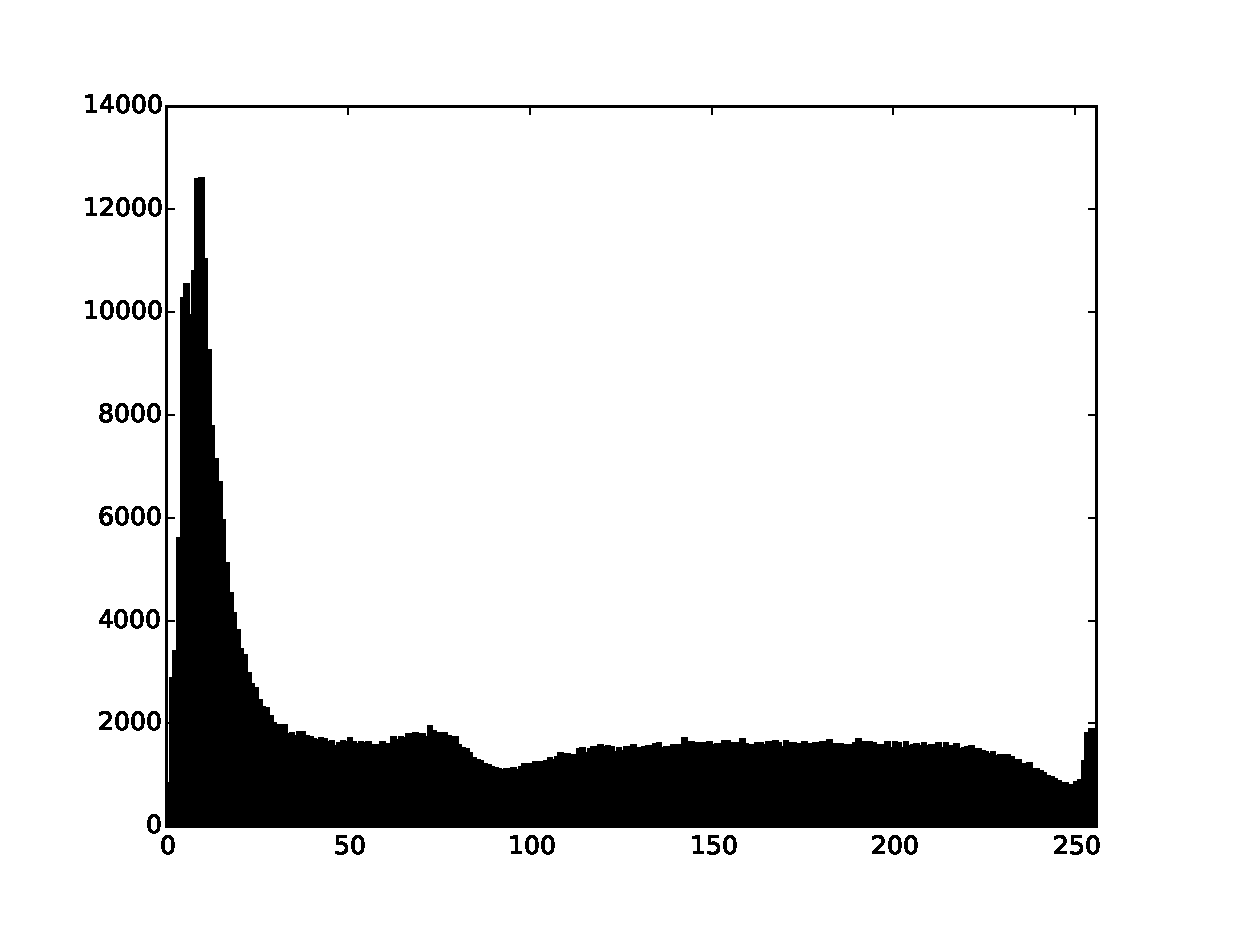
\includegraphics[width=0.520\linewidth]{bilder/moon_hist.eps}
\end{figure}
\end{frame}

\begin{frame}{\insertsubsection}
\begin{figure}[T]
  \centering
  \includegraphics[width=0.470\textwidth]{bilder/uniformnoise.png}
  \hfill
  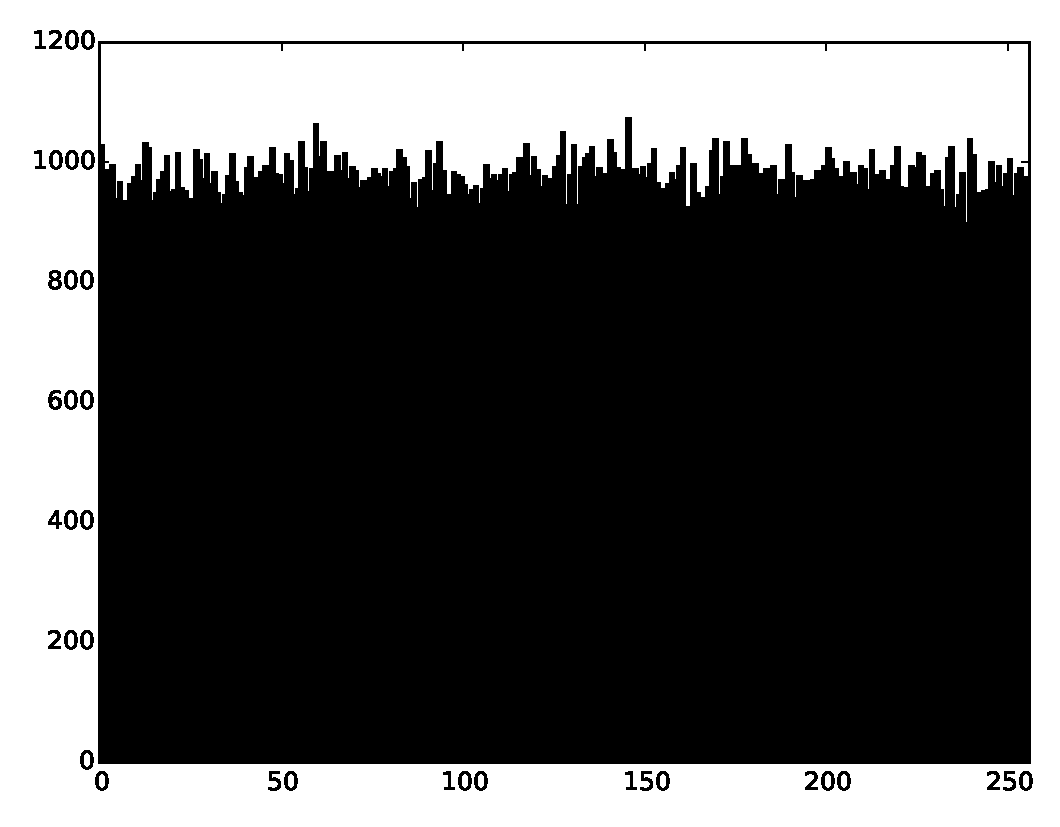
\includegraphics[width=0.520\linewidth]{bilder/uniformnoise_hist.eps}
\end{figure}
\end{frame}

%%%%%%%%%%%%%%%%%%%%%%%%%%%%%%%%%%%%%%%%%%%%%%%%%%%%%%%%%%%%

\begin{frame}[label=finalSlide]
  \label{LastPage}
  \begin{center}
    \vfill
    {\Large
    \textcolor{i6blue}{Danke für die Aufmerksamkeit!}
    }
     \vfill
     \inserttitle
    \vfill
    {\Large \insertauthor}
    \vfill
    \email{}
  \end{center}
\end{frame}

\end{document}
